\section{问题重述}

\subsection{研究背景}

随着"双碳"战略的深入推进，新能源大规模并网消纳难的问题日益凸显\cite{ref1}。绿电直连项目为探索促进新能源就近消纳提供了新路径，其中并网型项目作为整体接入公共电网，与公共电网形成清晰的物理界面与责任界面。国家发展改革委、国家能源局发布的《关于有序推动绿电直连发展有关事项的通知》对绿电直连项目的多项运行指标提出了明确要求，包括新能源自发自用电量占总可用发电量比例（要求大于60\%）、总用电量绿电比例（要求大于30\%）以及新能源上网电量占总可用发电量比例（要求小于20\%）。

"绿电—绿氢—绿氨"一体化绿电直连化工园区正在成为解决新能源消纳和化工行业深度脱碳的重要路径\cite{ref10}。由于氨相较于氢更易于储运，电氢氨一体化园区将风光发电、电解制氢、合成氨生产有机结合，形成了从清洁能源到绿色化工产品的完整产业链\cite{ref4}。

\subsection{问题概述}

本文研究的绿电直连型电氢氨园区包含风力发电（40 MW）、光伏发电（64 MW）、碱性电解槽（ALKEL）、质子交换膜电解槽（PEMEL）、合成氨装置及常规电负荷等组成部分。园区初始制氨产能为36吨/日，风光发电优先供给区域内制氢、制氨负荷以及本地电负荷，不足电量从外部电网购电，余电可上网。园区能量流向架构如图\ref{fig:energy_flow}所示。

\begin{figure}[H]
\centering
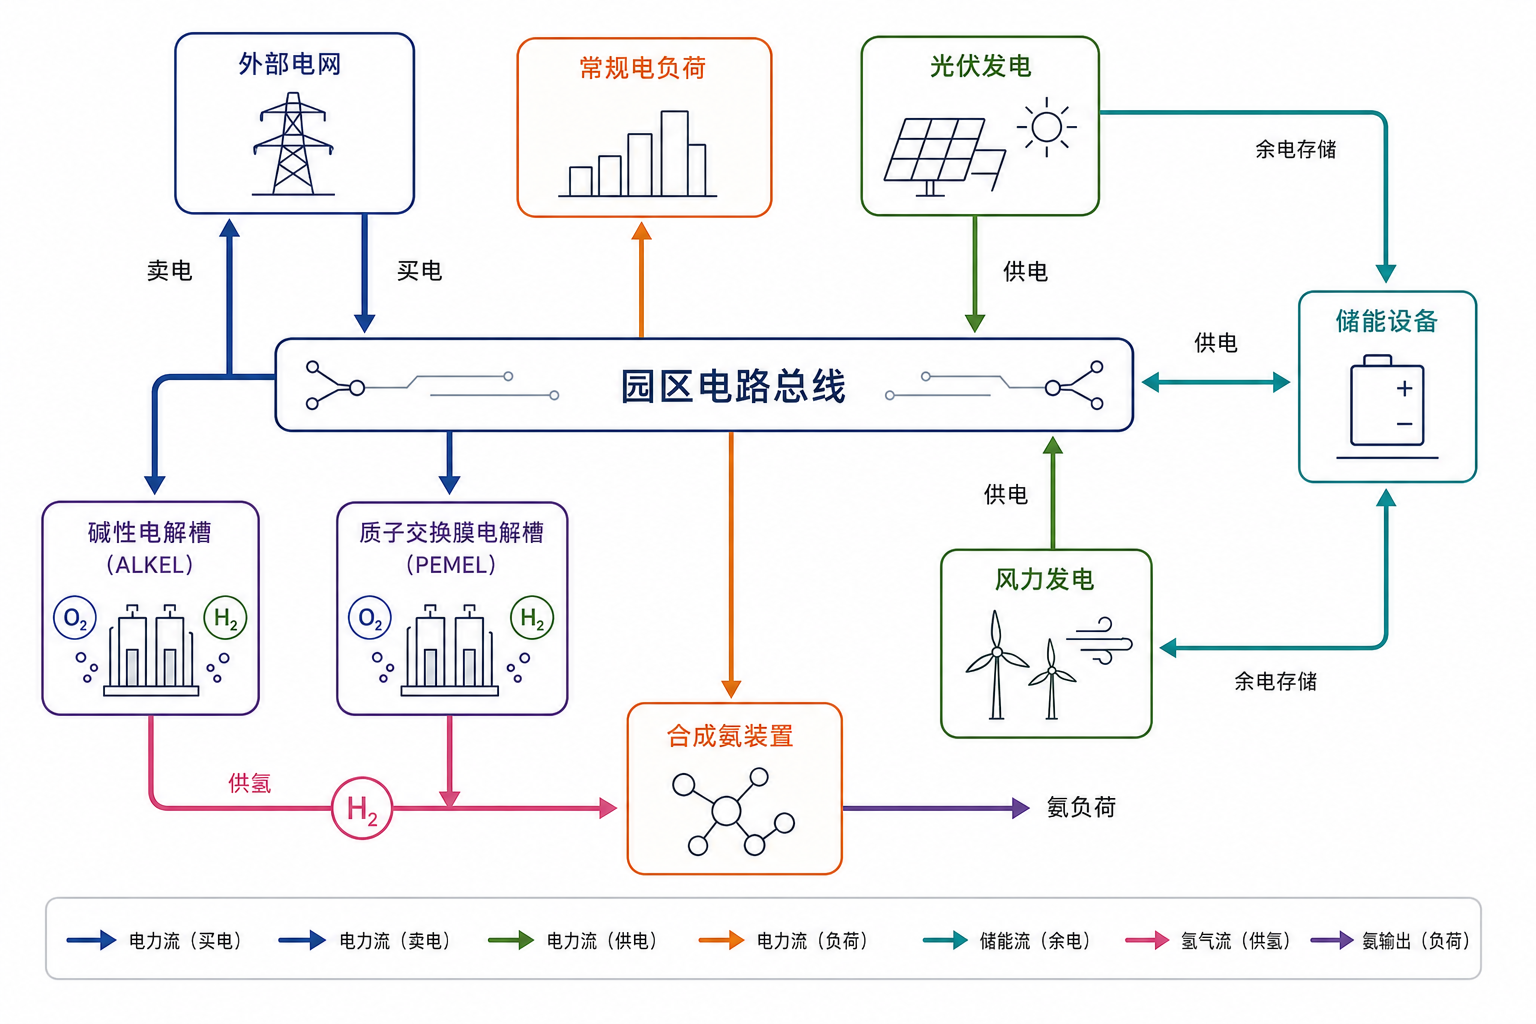
\includegraphics[width=0.8\linewidth]{ChatGPT Image 2026年5月23日 17_21_10.png}
\caption{绿电直连型电氢氨园区能量流向架构图}\label{fig:energy_flow}
\end{figure}

风电和光伏发电经汇流后，优先供给电解制氢设备（ALKEL和PEMEL）、合成氨装置以及园区常规电负荷。当风光出力超过园区总用电需求时，余电通过联网线路上网；当风光出力不足时，从外部电网购电补充。电解槽将电能转化为氢气，合成氨装置将氢气与氮气合成为氨产品。需要解决以下五个核心问题：

（1）在电解槽与合成氨装置每日满负荷连续运行条件下，计算园区典型日各项功率曲线和运行指标，分析绿电直连指标的满足情况。

（2）当园区制氨产能增至72吨/日时，电氢氨装置仅有全额开机和停机两种运行方式，需要确定不同产量水平下成本最低的生产时段安排，并在24种风光出力场景下统计分析全年运行指标。

（3）在电氢氨装置功率连续可调（下限为10\%）的条件下，对24种风光组合出力场景进行最优功率调度，并与问题二的离散调节结果进行对比分析。

（4）园区离网运行时，分析无储能和有储能两种情况下的制氨产量与经济性，确定最优储能配置方案，并对比离网与联网两种运行模式的经济性。

（5）分析绿电园区容量渗透率显著提高后对电力系统运行的影响，并提出推动绿电直连园区发展的政策建议。

\begin{figure}[H]
    \centering
    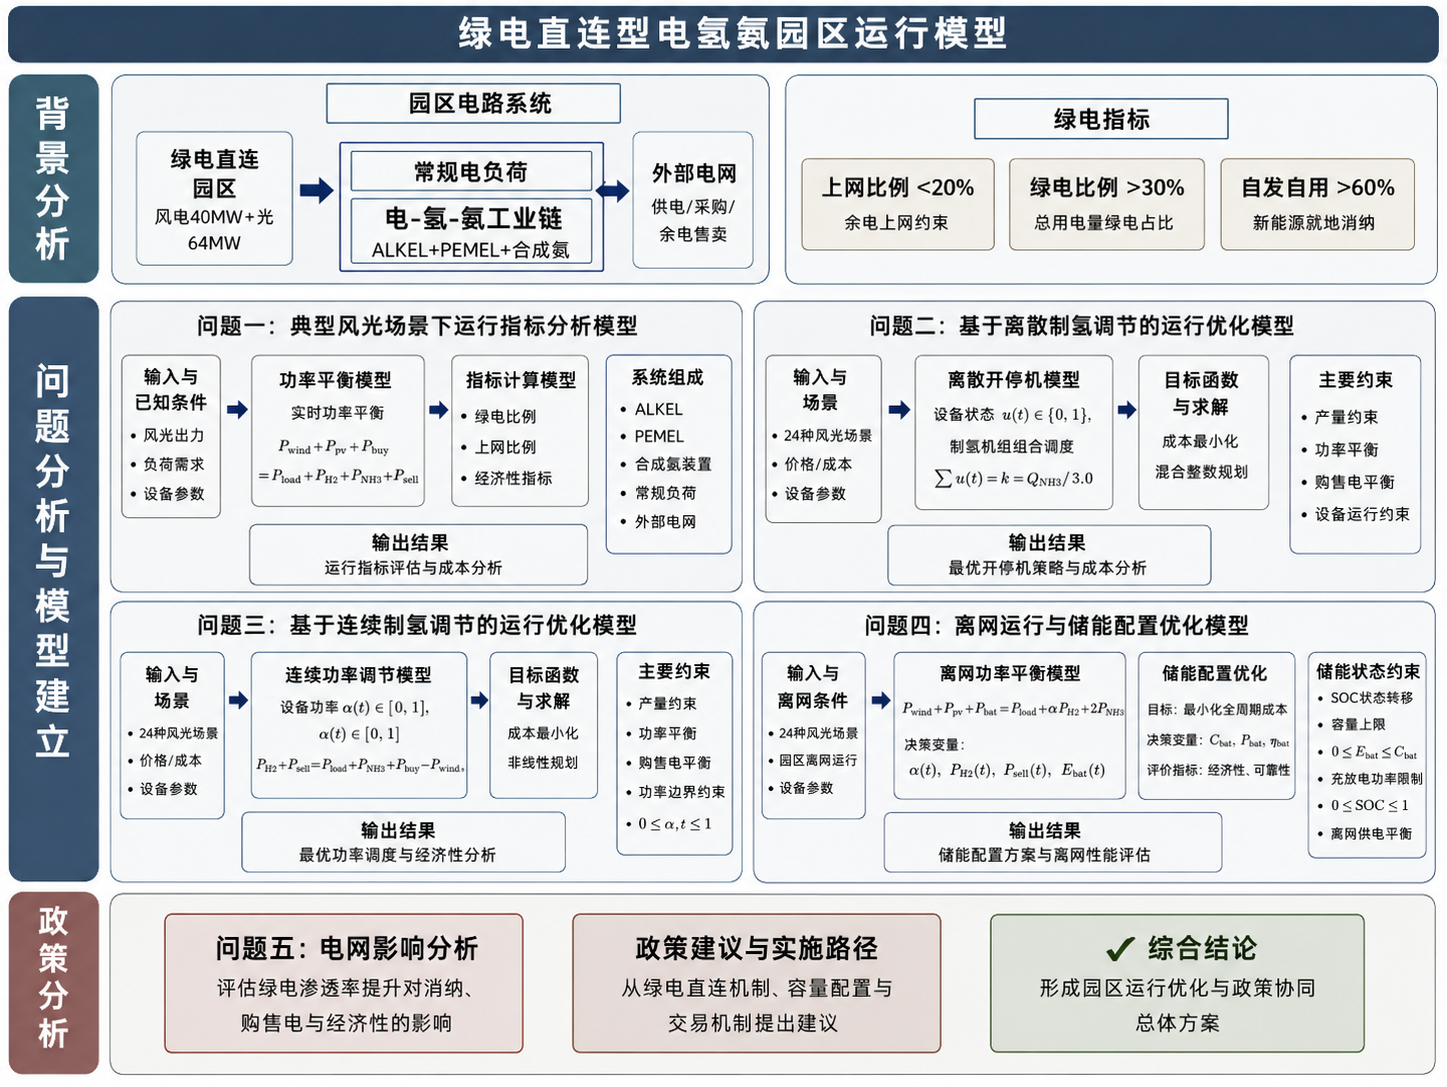
\includegraphics[width=1.0\linewidth]{ChatGPT Image 2026年5月24日 20_25_00.png}
    \caption{绿电直连型电氢氨园区优化运行整体技术路线图}\label{fig:roadmap}
\end{figure}

本文围绕上述五个问题，综合运用功率平衡分析、混合整数线性规划（MILP）、线性规划（LP）以及参数扫描优化等方法，系统研究了绿电直连型电氢氨园区在不同运行模式下的最优调度策略与经济性能（图\ref{fig:roadmap}）。
